\documentclass[11pt,a4paper]{article}
\usepackage[margin=2.3cm]{geometry}
\usepackage{amsmath,amssymb,bm}
\usepackage{siunitx}
\usepackage{booktabs}
\usepackage{graphicx}
\usepackage{tikz}
\usetikzlibrary{arrows.meta,calc,positioning,patterns}
\usepackage{pgfplots}
\pgfplotsset{compat=1.17}
\usepackage{enumitem}
\usepackage{float}
\tikzset{capt/.style={text width=5.2cm,align=center}}
\usepackage[colorlinks=true,linkcolor=blue!60!black,urlcolor=blue!60!black]{hyperref}
\usepackage{fancyhdr}
\usepackage{tcolorbox}
\tcbuselibrary{skins,breakable}
\sisetup{per-mode=symbol,detect-all}
\DeclareSIUnit{\MParm}{MPa\,\ensuremath{\sqrt{\text{m}}}}

\newtcolorbox{keybox}[1]{title={#1},colback=blue!4,colframe=blue!50!black,fonttitle=\bfseries,breakable}
\newtcolorbox{examplebox}[1]{title={#1},colback=green!4,colframe=green!40!black,fonttitle=\bfseries,breakable}
\newtcolorbox{aerobox}[1]{title={#1},colback=orange!5,colframe=orange!60!black,fonttitle=\bfseries,breakable}

\pagestyle{fancy}
\fancyhf{}
\lhead{
\includegraphics[height=0.6cm]{logos/itu_logo_laci.pdf}\ \ UCK 364E Design of Machine Elements}
\setlength{\headheight}{20pt}
\rhead{Lecture 3 -- Notes}
\cfoot{\thepage}

\title{\textbf{UCK 364E Design of Machine Elements}\\[4pt]
\Large Lecture 3: Fracture Mechanics, Fatigue Strength and Damage Tolerance\\[2pt]
\large Stress intensity, toughness, crack growth, residual strength and inspection intervals}
\author{Prof.\ Dr.\ Onur Tunçer\\ Department of Aeronautical Engineering, Istanbul Technical University}
\date{Fall 2026}

\begin{document}
\maketitle

\section*{Learning objectives}
By the end of this lecture you should be able to
\begin{enumerate}[nosep]
  \item explain why a strength-of-materials stress calculation fails at a crack tip, and what replaces it;
  \item compute the stress intensity factor $K_{\mathrm{I}}=\beta\sigma\sqrt{\pi a}$ for the standard configurations and find $\beta$ for a geometry from a handbook;
  \item state the fracture criterion $K_{\mathrm{I}}=K_{\mathrm{Ic}}$, compute the critical crack length, and explain the plane-stress/plane-strain thickness requirement;
  \item explain the three regimes of the $\mathrm{d}a/\mathrm{d}N$ curve, use the Paris law, and integrate it to a crack-growth life;
  \item construct a residual-strength diagram and read the critical crack size off it;
  \item derive an inspection interval from a crack-growth curve and a detectable crack size, and explain the role of the probability of detection;
  \item state what safe-life, fail-safe and damage tolerance require of the designer, and where each is used;
  \item relate all of this to CS-25.571 and to the Comet and Aloha case studies.
\end{enumerate}

\section{Where the previous lecture stopped}

Lecture~2 predicted the number of cycles to \emph{initiate} a crack: S--N for long lives, $\varepsilon$--N for short ones at notches. Both methods assume that the material starts out sound and end their usefulness at the moment a small crack appears.

That is not how aircraft structure is treated. Three facts force a different approach:

\begin{enumerate}[nosep]
  \item \textbf{Real structure contains flaws from the start} --- inclusions, scratches, burrs at drilled holes, corrosion pits, the torn edge of a punched rivet hole. The initiation phase may be absent entirely.
  \item \textbf{The scatter in initiation life is enormous}, a factor of ten or more, while crack \emph{growth} is far more repeatable. Predictions built on growth are more trustworthy.
  \item \textbf{A crack is survivable if you find it.} The entire modern philosophy is to accept that cracks will exist and to schedule inspections so that each one is found before it becomes dangerous.
\end{enumerate}

\begin{keybox}{The question changes}
Lecture 2 asked: \emph{how long until a crack appears?} \\
Lecture 3 asks: \emph{given that a crack exists, how long until it is dangerous --- and how often must I look?}
\end{keybox}

\section{Why ordinary stress analysis fails at a crack}

Consider an elliptical hole of semi-axes $a$ and $b$ in a wide plate under remote tension $\sigma$. The elastic stress concentration at the end of the major axis is
\begin{equation}
  K_t = 1+2\frac{a}{b} = 1+2\sqrt{\frac{a}{\rho}},
\end{equation}
where $\rho=b^2/a$ is the root radius. A circular hole ($a=b$) gives the familiar $K_t=3$. But as the ellipse is flattened into a crack, $\rho\to0$ and $K_t\to\infty$. The elasticity solution says the stress at a sharp crack tip is infinite \emph{whatever} the applied load.

An infinite stress cannot be compared with an allowable. Yet cracked structures plainly do carry load, and identical cracks in the same material fail at the same applied stress. Something other than the peak stress must be controlling fracture.

The resolution, due to Irwin, is to characterise not the peak value but the \emph{intensity} of the whole crack-tip stress field. Near the tip of a crack in a linear elastic body the stresses have the universal form
\begin{equation}
  \sigma_{ij}(r,\theta)=\frac{K}{\sqrt{2\pi r}}\,f_{ij}(\theta)+\dots
  \label{eq:field}
\end{equation}
The $r^{-1/2}$ singularity and the angular functions $f_{ij}(\theta)$ are the same for every crack in every body. All of the geometry and loading is contained in the single scalar $K$, the \textbf{stress intensity factor}. Two different cracked components with the same $K$ have the same crack-tip conditions and behave the same way --- that is the whole of linear elastic fracture mechanics in one sentence.

\begin{center}
\begin{tikzpicture}[scale=1.0,>=Stealth,font=\scriptsize]
\begin{scope}
\fill[blue!10] (0,0) rectangle (4.6,3.0);
\draw[thick] (0,0) rectangle (4.6,3.0);
\draw[line width=1.4pt] (1.0,1.5) -- (2.6,1.5);
\fill (2.6,1.5) circle (1.6pt);
\draw[->] (2.6,1.5) -- (3.5,2.1) node[midway,above,sloped] {$r$};
\draw (3.1,1.5) arc (0:33:0.5); \node at (3.25,1.72) {$\theta$};
\foreach \y in {0.3,0.75,...,2.9} {\draw[->,blue!55!black] (-0.75,\y) -- (-0.05,\y); \draw[->,blue!55!black] (5.35,\y) -- (4.65,\y);}
\node[blue!55!black,anchor=east] at (-0.85,1.5) {$\sigma$};
\draw[<->] (1.0,1.15) -- (2.6,1.15) node[midway,below] {$a$};
\node[anchor=north] at (2.3,-0.2) {a crack in a plate};
\end{scope}
\begin{scope}[xshift=7.4cm]
\draw[->] (0,0) -- (4.6,0) node[right] {$r$};
\draw[->] (0,0) -- (0,3.0) node[above] {$\sigma_{yy}$};
\draw[domain=0.22:4.3,samples=120,thick,red!70!black] plot (\x,{1.25/sqrt(\x)});
\draw[dashed] (0,0.6) -- (4.4,0.6) node[right,font=\tiny] {remote $\sigma$};
\node[red!70!black,anchor=west] at (1.4,2.2) {$\sigma_{yy}=\dfrac{K_{\mathrm I}}{\sqrt{2\pi r}}$};
\fill[gray!30,opacity=0.6] (0,0) rectangle (0.5,3.0);
\node[anchor=south,font=\tiny,align=center] at (0.25,3.0) {plastic\\ zone};
\node[anchor=north] at (2.3,-0.25) {the crack-tip field};
\end{scope}
\end{tikzpicture}
\end{center}

\subsection{The three modes}
Cracks can be loaded in three independent ways: \textbf{Mode I} (opening, tension normal to the crack plane), \textbf{Mode II} (in-plane shear/sliding) and \textbf{Mode III} (out-of-plane shear/tearing). Mode I dominates in practice, because a crack under mixed loading turns to grow normal to the maximum principal stress and so converts itself into a Mode I crack. We will work only with $K_{\mathrm{I}}$.

\section{The stress intensity factor}

For every configuration the stress intensity factor takes the form
\begin{equation}
  \boxed{\;K_{\mathrm{I}}=\beta\,\sigma\sqrt{\pi a}\;}
  \label{eq:K}
\end{equation}
with units \si{\MParm}. Here $\sigma$ is the \emph{nominal} (remote, uncracked) stress, $a$ is the crack size, and $\beta$ is a dimensionless geometry factor of order one, tabulated in handbooks (Tada, Murakami, NASGRO) for hundreds of configurations.

\begin{center}\small
\begin{tabular}{@{}llp{6.2cm}@{}}
\toprule
Configuration & $\beta$ & Note \\
\midrule
Central crack $2a$, infinite plate & $1.00$ & the reference case \\
Edge crack $a$, semi-infinite plate & $1.12$ & the free edge relieves constraint \\
Two symmetric cracks at a hole, infinite plate & $\approx1.0$ (for $a\gg R$) & $a$ measured from the hole centre \\
Short crack at a hole, $a\ll R$ & $\approx1.12\times3=3.4$ & the crack lies in the $K_t$ field of the hole \\
Embedded penny crack, radius $a$ & $2/\pi=0.64$ & fully constrained \\
Surface semi-elliptical crack & $\approx0.7$--$1.1$ & depends on $a/c$ and $a/t$ \\
Central crack in a plate of width $W$ & $\sqrt{\sec(\pi a/W)}$ & finite-width correction \\
\bottomrule
\end{tabular}
\end{center}

\begin{keybox}{Three things students get wrong}
\textbf{1.} $K$ is not $K_t$. The stress concentration factor $K_t$ is dimensionless and describes a \emph{notch}; the stress intensity factor $K_{\mathrm{I}}$ has units of \si{\MParm} and describes a \emph{crack}. \\
\textbf{2.} $\sigma$ in Eq.~\eqref{eq:K} is the stress that would exist \emph{without} the crack, not a local stress. \\
\textbf{3.} $K$ grows with $\sqrt{a}$: doubling the crack length raises $K$ by only 41\%, which is why crack growth is slow at first and catastrophic at the end.
\end{keybox}

\subsection{The plastic zone and when LEFM is valid}
Equation~\eqref{eq:field} predicts infinite stress, so the material must yield in a small region at the tip. Irwin's estimate of its size is
\begin{equation}
  r_p=\frac{1}{2\pi}\left(\frac{K_{\mathrm{I}}}{\sigma_y}\right)^{2}\ \ \text{(plane stress)},\qquad
  r_p=\frac{1}{6\pi}\left(\frac{K_{\mathrm{I}}}{\sigma_y}\right)^{2}\ \ \text{(plane strain)} .
\end{equation}
Linear elastic fracture mechanics is valid only while this zone is small compared with the crack and the remaining ligament --- \emph{small-scale yielding}. A useful rule: the crack length, the ligament and the thickness should each exceed $2.5(K/\sigma_y)^2$. When they do not, LEFM is invalid and elastic--plastic methods ($J$-integral, CTOD) are needed; thin aluminium sheet in a fuselage is often in this regime, which is why residual strength there is treated with the crack-tip opening angle or with an $R$-curve rather than a single toughness value.

\section{Fracture toughness}

Fracture occurs when the crack-tip field reaches the material's capacity to resist it:
\begin{equation}
  K_{\mathrm{I}}=K_{\mathrm{Ic}} .
\end{equation}
$K_{\mathrm{Ic}}$ is the \textbf{plane-strain fracture toughness}, a material property measured to ASTM E399 on a specimen thick enough to guarantee plane strain, namely
\begin{equation}
  B,\;a,\;(W-a)\ \ge\ 2.5\left(\frac{K_{\mathrm{Ic}}}{\sigma_y}\right)^{2}.
\end{equation}

Thickness matters because it controls constraint. A thin sheet is free to contract through the thickness, so the tip is in plane stress, the plastic zone is large, and the apparent toughness $K_c$ is high. A thick section prevents that contraction, the tip is in plane strain, the plastic zone is small, and the toughness falls to its minimum, conservative value $K_{\mathrm{Ic}}$. Beyond the transition thickness it stops falling. \emph{Design with $K_{\mathrm{Ic}}$ unless you can justify the thin-section value by test.}

\begin{center}\small
\begin{tabular}{@{}lS[table-format=4]S[table-format=2.0]S[table-format=2.1]p{4.8cm}@{}}
\toprule
Material & {$\sigma_y$ (MPa)} & {$K_{\mathrm{Ic}}$ (MPa$\sqrt{\text{m}}$)} & {$a_c$ (mm)$^{*}$} & Comment \\
\midrule
2024-T3 sheet & 289 & 37 & 46.3 & damage tolerant; fuselage skin \\
7075-T6 & 462 & 24 & 19.5 & high strength, low toughness \\
7075-T73 & 400 & 31 & 32.5 & overaged: toughness and SCC bought with strength \\
7050-T7451 plate & 427 & 33 & 36.8 & thick fittings \\
Ti-6Al-4V (ann.) & 827 & 75 & 190.1 & excellent combination \\
4340 (1800 MPa) & 1517 & 50 & 84.5 & high strength, modest toughness \\
300M (1900 MPa) & 1600 & 65 & 142.8 & landing gear; toughness is why \\
\bottomrule
\end{tabular}
\end{center}
{\footnotesize *$a_c$ = critical crack length for a central crack ($\beta=1$) at a nominal stress of $\sigma=0.5\sigma_y$: $a_c=(1/\pi)(K_{\mathrm{Ic}}/\beta\sigma)^2$. Classroom values only.}

\begin{aerobox}{The strength--toughness trade, quantified}
Compare 7075-T6 and 2024-T3 in the table. The 7075 is 60\% stronger, so you could run it at a higher stress --- but its critical crack is less than half as long, and at equal stress the difference is larger still. This is exactly why the \emph{lower} wing surface and the fuselage, which are tension-fatigue critical and inspected, are 2024, while the \emph{upper} wing surface, which is compression critical, is 7075. The choice is not ``which alloy is better'' but ``which failure mode governs here''.
\end{aerobox}

\section{Fatigue crack growth}

Under cyclic loading the crack-tip field also cycles, with range
\begin{equation}
  \Delta K = K_{\max}-K_{\min}=\beta\,\Delta\sigma\sqrt{\pi a},\qquad R=\frac{K_{\min}}{K_{\max}} .
\end{equation}
Paris observed that the growth per cycle correlates with $\Delta K$, and plotting $\log(\mathrm{d}a/\mathrm{d}N)$ against $\log\Delta K$ produces the sigmoidal curve below with three regimes.

\begin{figure}[H]\centering
\begin{tikzpicture}
\begin{loglogaxis}[width=11.2cm,height=6.4cm,xlabel={$\Delta K$ (MPa$\sqrt{\text{m}}$)},ylabel={$\mathrm{d}a/\mathrm{d}N$ (m/cycle)},
 xmin=2,xmax=90,ymin=1e-11,ymax=1e-5,grid=both,grid style={gray!20},
 xtick={2,3,5,10,20,50},xticklabels={2,3,5,10,20,50},
 label style={font=\footnotesize},tick label style={font=\footnotesize}]
\addplot[very thick,blue!60!black,domain=3.06:54.2,samples=400]
  {3e-12*x^3*sqrt(1-3/x)/sqrt(1-x/55)};
\draw[gray,dashed] (axis cs:3.1,1e-11) -- (axis cs:3.1,1e-5);
\draw[gray,dashed] (axis cs:55,1e-11) -- (axis cs:55,1e-5);
\node[font=\scriptsize,anchor=south west] at (axis cs:2.3,3e-11) {$\Delta K_{th}$};
\node[font=\scriptsize,anchor=south east] at (axis cs:85,3e-11) {$K_{\mathrm{Ic}}$};
\node[font=\scriptsize,align=center] at (axis cs:3.9,3e-8) {I\\ threshold};
\node[font=\scriptsize,align=center,anchor=west] at (axis cs:12,4e-10) {II\ \ Paris r\'egime\\ $\mathrm{d}a/\mathrm{d}N=C(\Delta K)^m$};
\node[font=\scriptsize,align=center] at (axis cs:68,2e-7) {III\\ unstable};
\end{loglogaxis}
\end{tikzpicture}
\caption{The fatigue crack growth rate curve. Regime I: below the threshold $\Delta K_{th}$ cracks do not propagate. Regime II: the straight Paris line, where most of the life is spent and where design calculations are made. Regime III: $K_{\max}$ approaches $K_{\mathrm{Ic}}$ and growth runs away to fracture.}
\label{fig:dadn}
\end{figure}

\subsection{The Paris law}
In regime II,
\begin{equation}
  \boxed{\;\frac{\mathrm{d}a}{\mathrm{d}N}=C\,(\Delta K)^{m}\;}
  \label{eq:paris}
\end{equation}
with $m\approx 2.5$--$4$ for metals ($\approx3$ for steels, $\approx3$--$4$ for aluminium alloys) and $C$ a material constant whose units depend on $m$. Note what the exponent means: because $\Delta K\propto\sqrt{a}$, the growth rate goes as $a^{m/2}$. With $m=4$ the rate is proportional to $a^2$ --- a crack ten times longer grows a hundred times faster. That is the shape of the $a$--$N$ curve you met in the Comet handout.

\subsection{Integrating to a life}
Separating variables in Eq.~\eqref{eq:paris} and integrating from an initial crack $a_i$ to a final crack $a_f$:
\begin{equation}
  N_f=\int_{a_i}^{a_f}\frac{\mathrm{d}a}{C\left(\beta\Delta\sigma\sqrt{\pi a}\right)^{m}} .
\end{equation}
If $\beta$ is taken as constant and $m\neq2$ this integrates in closed form:
\begin{equation}
  \boxed{\;N_f=\frac{2}{(m-2)\,C\,\beta^{m}\,\Delta\sigma^{m}\,\pi^{m/2}}
  \left[\frac{1}{a_i^{(m-2)/2}}-\frac{1}{a_f^{(m-2)/2}}\right]\;}
  \label{eq:life}
\end{equation}
Three consequences are worth stating explicitly:
\begin{itemize}[nosep]
  \item The life is dominated by $a_i$. Halving the initial flaw size is worth far more than doubling the final one.
  \item The final crack size barely matters: with $m=4$ the second term in the bracket is usually negligible. You can often take $a_f\to\infty$ and lose nothing.
  \item Life scales as $\Delta\sigma^{-m}$. A 10\% reduction in stress range buys about 46\% more life at $m=4$.
\end{itemize}
In practice $\beta$ varies with $a$ and the integral is done numerically, cycle by cycle, with the spectrum of Lecture~2 --- which is what NASGRO and AFGROW do.

\subsection{Mean stress, closure and retardation}
Growth rate depends on $R$ as well as $\Delta K$: at higher mean stress the crack is open for more of the cycle and grows faster. The Forman and NASGRO equations add this dependence explicitly. The physical mechanism is \textbf{crack closure}: the plastic wake left behind the advancing tip props the crack open, so that part of the nominal $\Delta K$ does no damage, and only an effective range $\Delta K_{\text{eff}}$ drives growth.

Closure also explains \textbf{retardation}: a single large overload creates an oversized plastic zone that the crack must grow through, and growth slows or stops for thousands of cycles afterwards. Retardation is real and is sometimes worth tens of percent of life --- but it is normally \emph{ignored} in certification, because it is non-conservative to rely on and because a high-low sequence can equally produce acceleration.

\section{Residual strength and the critical crack}

As a crack grows, the load the structure can still carry falls. Plotting that remaining capability against crack length gives the \textbf{residual strength diagram}, the central picture of damage tolerance.

\begin{figure}[H]\centering
\begin{tikzpicture}
\begin{axis}[width=11.6cm,height=6.2cm,xlabel={crack length $a$ (mm)},ylabel={residual strength (MPa)},
 xmin=0,xmax=120,ymin=0,ymax=330,grid=both,grid style={gray!20},
 label style={font=\footnotesize},tick label style={font=\footnotesize}]
% net section yield line
\addplot[thick,green!45!black,domain=0:120,samples=2]{289*(1-x/260)};
% fracture line K=Kic
\addplot[very thick,red!70!black,domain=4:120,samples=120]{37/sqrt(3.1416*x/1000)};
% limit and ultimate
\draw[dashed,black] (axis cs:0,116) -- (axis cs:120,116);
\node[font=\scriptsize,anchor=south east] at (axis cs:118,118) {design ultimate stress};
\draw[dashed,black] (axis cs:0,77) -- (axis cs:120,77);
\node[font=\scriptsize,anchor=north east] at (axis cs:118,74) {limit stress};
% critical crack sizes, read off the fracture curve
\draw[gray,dashed] (axis cs:32.4,0) -- (axis cs:32.4,116);
\fill (axis cs:32.4,116) circle (1.8pt);
\node[font=\scriptsize,anchor=south west,align=left] at (axis cs:33,128) {$a_c=\SI{32}{mm}$\\ at ultimate};
\draw[gray,dashed] (axis cs:73.5,0) -- (axis cs:73.5,77);
\fill (axis cs:73.5,77) circle (1.8pt);
\node[font=\scriptsize,anchor=south,align=center] at (axis cs:73.5,12) {$a_c=\SI{73}{mm}$ at limit};
\node[font=\scriptsize,red!70!black,anchor=west] at (axis cs:17,235) {fracture, $K_{\mathrm I}=K_{\mathrm{Ic}}$};
\node[font=\scriptsize,green!45!black,anchor=east] at (axis cs:118,205) {net-section yield};
\end{axis}
\end{tikzpicture}
\caption{Residual strength diagram for a 2024-T3 panel ($K_{\mathrm{Ic}}=\SI{37}{\MParm}$, $\sigma_y=\SI{289}{MPa}$, central crack, $\beta=1$). The structure is governed by net-section yield when the crack is short and by fracture when it is long. The critical crack size depends on the stress level you require the cracked structure to survive --- which is a certification decision, not a material property.}
\label{fig:residual}
\end{figure}

\begin{keybox}{What ``critical'' means}
There is no single critical crack length. There is a crack length that is critical \emph{at a stated stress}. CS-25.571 requires the cracked structure to carry a specified residual-strength load --- commonly limit load, or a defined fraction of it, depending on the structural category and the inspection programme. Choose the stress first, then read $a_c$ off the diagram.
\end{keybox}

\section{The inspection interval --- where it all comes together}

This is the practical pay-off of the lecture, and the reason damage tolerance replaced safe life for transport structure.

\begin{enumerate}[nosep]
  \item Assume an initial flaw $a_0$. Typically the largest flaw that could escape manufacturing inspection, e.g.\ \SI{1.27}{mm} (0.05\,in) at a fastener hole, by convention.
  \item Compute $a_c$ from the residual-strength requirement (Figure~\ref{fig:residual}).
  \item Integrate the growth law over the flight spectrum to get the curve $a(N)$ from $a_0$ to $a_c$. Call that total crack-growth life $N_c$.
  \item Determine the \textbf{detectable} crack size $a_{\mathrm{det}}$ for the inspection method you intend to specify, at the required probability of detection.
  \item The usable window is from $a_{\mathrm{det}}$ to $a_c$. Let $N_{\mathrm{window}}$ be the number of flights to cross it.
  \item Set the repeat inspection interval at $N_{\mathrm{window}}/n$, with $n=2$ or more, so that at least two inspections occur while the crack is detectable but not yet critical.
\end{enumerate}

\begin{figure}[H]\centering
\begin{tikzpicture}
\begin{axis}[width=12cm,height=6.0cm,xlabel={flights $N$},ylabel={crack length $a$},
 xmin=0,xmax=1.02,ymin=0,ymax=1.05,xtick=\empty,ytick=\empty,axis lines=left,
 label style={font=\footnotesize}]
\addplot[very thick,red!70!black,domain=0:0.965,samples=240]{0.045+0.0016*exp(6.6*x)};
\draw[dashed] (axis cs:0,0.93) -- (axis cs:1.0,0.93);
\node[font=\scriptsize,anchor=north west] at (axis cs:0.02,0.92) {$a_c$ --- residual strength lost};
\draw[dashed] (axis cs:0,0.33) -- (axis cs:1.0,0.33);
\node[font=\scriptsize,anchor=south west] at (axis cs:0.02,0.34) {$a_{\mathrm{det}}$ --- detectable by the chosen NDT};
\draw[dashed] (axis cs:0,0.047) -- (axis cs:1.0,0.047);
\node[font=\scriptsize,anchor=south west] at (axis cs:0.02,0.06) {$a_0$ --- assumed manufacturing flaw};
% detectable / critical crossings
\fill (axis cs:0.785,0.33) circle (1.8pt);
\fill (axis cs:0.957,0.93) circle (1.8pt);
\draw[gray,dashed] (axis cs:0.785,0) -- (axis cs:0.785,0.33);
\draw[gray,dashed] (axis cs:0.957,0) -- (axis cs:0.957,0.93);
% window
\draw[<->,thick] (axis cs:0.785,0.60) -- (axis cs:0.957,0.60);
\node[font=\scriptsize,anchor=south east,align=right] at (axis cs:0.78,0.57) {$N_{\mathrm{window}}$};
% inspections
\draw[blue!60!black,very thick] (axis cs:0.800,0.0) -- (axis cs:0.800,0.10);
\draw[blue!60!black,very thick] (axis cs:0.858,0.0) -- (axis cs:0.858,0.10);
\draw[blue!60!black,very thick] (axis cs:0.916,0.0) -- (axis cs:0.916,0.10);
\node[font=\scriptsize,blue!60!black,anchor=east] at (axis cs:0.785,0.05) {inspections};
\end{axis}
\end{tikzpicture}
\caption{Setting an inspection interval. Almost the whole crack-growth life is spent below the detectable size; the usable window is the short, steep final part. The interval is the window divided by the number of inspection opportunities required, so a crack that becomes detectable just after one inspection is still found at the next --- with margin --- before it reaches $a_c$.}
\label{fig:interval}
\end{figure}

\subsection{Detectability is a design parameter}
$a_{\mathrm{det}}$ is not a constant of nature; it depends on the method, the access and the inspector:

\begin{center}\small
\begin{tabular}{@{}llp{6.6cm}@{}}
\toprule
Method & Typical $a_{\mathrm{det}}$ & Notes \\
\midrule
General visual, in service & \SIrange{25}{50}{mm} & unaided, from a walkaround distance \\
Detailed visual, close & \SIrange{5}{15}{mm} & clean surface, good light, structure unloaded \\
Dye penetrant & \SIrange{2}{5}{mm} & surface-breaking only, surface must be accessible \\
Eddy current, surface & \SIrange{1}{2}{mm} & finds cracks under rivet heads --- the Aloha method \\
Ultrasonic & \SIrange{1}{3}{mm} & subsurface; needs couplant and a trained operator \\
X-ray & $\approx$2\% of thickness & poor for tight cracks normal to the beam \\
\bottomrule
\end{tabular}
\end{center}

Formally, detection is probabilistic: the \textbf{probability of detection} (POD) curve rises from zero to near unity with crack size, and the figure used in certification is typically the crack size detected with 90\% probability at 95\% confidence, written $a_{90/95}$. The designer's influence is real and direct: \emph{provide access}. A crack that can only be found by removing an engine will be inspected rarely and the interval will be driven to an uneconomic place --- or the part will have to be safe-life.

\begin{aerobox}{Why this is a \emph{design} lecture, not a materials lecture}
Everything on the inspection-interval list is something a designer controls: the initial flaw size (hole quality, cold expansion, finish), the stress range (sizing, load path), the critical crack size (material choice, tear straps, crack stoppers), the detectable size (choice of method and, above all, \emph{access}), and the number of load paths. A structure that is awkward to inspect is a design error, not a maintenance problem.
\end{aerobox}

\section{The three philosophies, properly}

\begin{description}[nosep,leftmargin=0.7cm,style=nextline]
  \item[Safe-life.] The part is assumed crack-free and is retired at a life demonstrated by test and analysis, divided by a scatter factor (typically 3--5 against a full-scale test). No inspection credit. Used where inspection is impractical or where a single crack is immediately catastrophic: landing-gear structure, engine discs, many rotorcraft dynamic components. The weakness is that the scatter factor is a guess about variability, and the F-111 wing carry-through failure in 1969 --- a safe-life structure that failed at 100 flight hours from a forging defect --- is the accident that discredited it for airframes.
  \item[Fail-safe.] The structure has multiple load paths, or crack-arrest features, so that after the complete failure of any one element the remainder still carries a specified load (commonly limit load) for long enough to be found. The Comet's successors, the dual-lug fitting from Lecture~1's error gallery, and the tear straps that saved the Aloha aircraft are all fail-safe thinking.
  \item[Damage tolerance.] Cracks are assumed present from the first flight. Growth is calculated, residual strength is demonstrated, and an inspection programme is derived --- as above. This is the default for transport-category metallic structure under CS-25.571, and the inspection programme is part of the certified design, not an afterthought.
\end{description}

\begin{keybox}{Widespread fatigue damage limits all of it}
Everything in this lecture assumes a \emph{single} dominant crack growing in otherwise sound structure. Aloha 243 showed that assumption failing: many small cracks on one rivet row, none individually detectable, linking up to produce a long crack in a few cycles. Residual strength then collapses far faster than single-crack analysis predicts. This is why the regulations added widespread fatigue damage and the \textbf{Limit of Validity} --- a cycle count beyond which the aircraft may not fly without further substantiation, however good its inspection record.
\end{keybox}

\section{Worked examples}

\begin{examplebox}{Example 3.1 --- Critical crack length in a fuselage skin}
A 2024-T3 fuselage skin carries a hoop stress of \SI{95}{MPa} at limit load. Take $K_{\mathrm{Ic}}=\SI{37}{\MParm}$ and treat a central through-crack with $\beta=1$.

Setting $K_{\mathrm{I}}=K_{\mathrm{Ic}}$ in Eq.~\eqref{eq:K}:
\[
a_c=\frac{1}{\pi}\left(\frac{K_{\mathrm{Ic}}}{\beta\sigma}\right)^{2}
=\frac{1}{\pi}\left(\frac{37}{95}\right)^{2}=\frac{0.1517}{\pi}=\SI{0.0483}{m}=\SI{48}{mm}.
\]
So a through-crack of about \SI{97}{mm} tip to tip ($2a_c$) is critical at limit load. That is a large, visible crack --- which is the point: 2024-T3 was chosen precisely so that the critical crack is big enough to find. Repeat the calculation for 7075-T6 at the same stress ($K_{\mathrm{Ic}}=\SI{24}{\MParm}$) and you get $a_c=\SI{20}{mm}$, less than half.

Check LEFM validity: $2.5(K/\sigma_y)^2=2.5(37/289)^2=\SI{41}{mm}$, which far exceeds the \SI{1.6}{mm} skin thickness. The sheet is therefore in \emph{plane stress}, not plane strain, so the real toughness is higher than $K_{\mathrm{Ic}}$ and this estimate is conservative --- but the proper treatment of a thin skin needs an $R$-curve, not a single number.
\end{examplebox}

\begin{examplebox}{Example 3.2 --- Crack growth life at a fastener hole}
A 7075-T6 lug is cycled with $\Delta\sigma=\SI{80}{MPa}$ at $R=0$. A corner crack of $a_i=\SI{1.27}{mm}$ is assumed at a fastener hole, this being the conventional non-detectable manufacturing flaw. Take $\beta=1.12$, and Paris constants $C=\SI{2.0e-11}{}$ and $m=3.5$ \emph{in units of \si{m/cycle} with $\Delta K$ in \si{\MParm}}. $K_{\mathrm{Ic}}=\SI{24}{\MParm}$.

\textbf{Final crack size.} Fracture when $K_{\max}=K_{\mathrm{Ic}}$; at $R=0$, $K_{\max}=\Delta K$, so
\[
a_f=\frac{1}{\pi}\left(\frac{K_{\mathrm{Ic}}}{\beta\,\Delta\sigma}\right)^{2}
=\frac{1}{\pi}\left(\frac{24}{1.12\times80}\right)^{2}=\SI{22.8}{mm}.
\]

\textbf{Life.} With $m=3.5$: $(m-2)=1.5$, $(m-2)/2=0.75$, $m/2=1.75$. Evaluate the denominator of Eq.~\eqref{eq:life}:
\[
(m-2)\,C\,\beta^{m}\,\Delta\sigma^{m}\,\pi^{m/2}
=1.5\times2.0\times10^{-11}\times1.487\times4.579\times10^{6}\times7.413
=1.514\times10^{-3}.
\]
And the bracket, with $a$ in metres:
\[
a_i^{-0.75}-a_f^{-0.75}=(0.00127)^{-0.75}-(0.02284)^{-0.75}=148.6-17.0=131.6 .
\]
Hence
\[
N_f=\frac{2\times131.6}{1.514\times10^{-3}}=1.74\times10^{5}\ \text{cycles}.
\]

Note how little the final crack size matters: the second term contributes only 11\% of the bracket. Had the crack been allowed to run to twice the length, the life would change by about 5\%. Had the \emph{initial} flaw been half as large, the life would roughly \emph{double}. This asymmetry is the single most important practical fact in the subject.
\end{examplebox}

\begin{keybox}{Units --- the most common error in this subject}
Crack-growth constants are published in at least four unit systems: $\mathrm{d}a/\mathrm{d}N$ in \si{m/cycle}, \si{mm/cycle} or in/cycle, and $\Delta K$ in \si{\MParm} or ksi$\sqrt{\text{in}}$. $C$ changes by orders of magnitude between them, and $m$ does not, so a wrong $C$ produces an answer that is wrong by a factor of $10^3$ and still looks plausible on a log plot.

\medskip
Two defences. First, state the unit system beside every $C$ you write down. Second, sanity-check: for aluminium alloys at $\Delta K=\SI{10}{\MParm}$, $\mathrm{d}a/\mathrm{d}N$ should come out at a few times $\SI{e-8}{m/cycle}$, i.e.\ tens of nanometres per cycle --- about one atomic spacing per cycle times a hundred. In the example above, $C(10)^{3.5}=\SI{6.3e-8}{m/cycle}$, which passes.
\end{keybox}

\begin{examplebox}{Example 3.3 --- Setting an inspection interval}
Continue Example 3.2. The lug is in a wing fitting that can be reached with an eddy-current probe, for which $a_{90/95}=\SI{2}{mm}$. The aircraft flies 1\,500 flights per year with one significant cycle per flight.

\textbf{Flights to reach the detectable size.} Using Eq.~\eqref{eq:life} from $a_i=\SI{1.27}{mm}$ to $a_{\mathrm{det}}=\SI{2}{mm}$:
\[
N(1.27\to2)=\frac{2\,(148.6-105.7)}{1.514\times10^{-3}}=5.67\times10^{4}\ \text{flights}.
\]
\textbf{Total crack-growth life.} $N(1.27\to22.8)=1.74\times10^{5}$ flights, from Example 3.2.

\textbf{Window.} $N_{\mathrm{window}}=1.74\times10^{5}-5.67\times10^{4}=1.17\times10^{5}$ flights.

\textbf{Interval.} With $n=2$ opportunities inside the window, the repeat interval is $1.17\times10^{5}/2=5.9\times10^{4}$ flights, about 39 years at this utilisation. The crack is detectable for two-thirds of its growth life, so this detail is comfortably inspectable and the programme will be set by the threshold for the \emph{first} inspection and by economics, not by this calculation.

\medskip
\textbf{Now change one thing.} Suppose the fitting is buried and can only be given a general visual inspection, $a_{\mathrm{det}}=\SI{25}{mm}$. But $a_c=\SI{22.8}{mm}$: the crack reaches critical size \emph{before} it becomes detectable. The window is negative and \textbf{no inspection interval exists}. The options are to redesign for lower stress or a tougher material (raising $a_c$), to provide access for a better method (lowering $a_{\mathrm{det}}$), to add a second load path and certify fail-safe, or to declare the part safe-life and retire it on a cycle count.

\medskip
This calculation costs ten minutes and decides whether a design is maintainable. Do it while the layout can still be changed.
\end{examplebox}

\section{Fatigue and fracture in the certification codes}

CS-25.571 and FAR 25.571 require a damage-tolerance evaluation of each part whose failure would be catastrophic, covering: the identification of principal structural elements, the assumed initial damage, crack growth under the service load spectrum, residual strength with the damage present, and the resulting inspection programme and thresholds --- all substantiated by analysis supported by test evidence. Where damage tolerance is impractical, a safe-life evaluation may be used instead, with a justified scatter factor. Widespread fatigue damage must be addressed and a Limit of Validity established. AMC 25.571 and FAA AC 25.571-1D give the accepted means of compliance; AC 25.571-1D is worth reading for its worked treatment of inspection thresholds.

\begin{aerobox}{Design levers for damage tolerance}
\begin{enumerate}[nosep]
  \item \textbf{Reduce the initial flaw.} Drilled and reamed holes instead of punched; cold expansion; deburring; better surface finish. The life integral is dominated by $a_i$.
  \item \textbf{Reduce the stress range.} Life goes as $\Delta\sigma^{-m}$, so a modest stress reduction buys a disproportionate life.
  \item \textbf{Increase the critical crack size.} A tougher alloy, thinner gauge in plane stress, tear straps and crack stoppers that arrest a running crack at a known boundary.
  \item \textbf{Make it inspectable.} Access panels, line of sight, a surface a probe can reach. This is a geometry decision made very early.
  \item \textbf{Add a second load path.} Fail-safe design removes the single-point dependency on finding the crack at all.
\end{enumerate}
\end{aerobox}

\section{Problems for self-study}
\begin{enumerate}[nosep]
  \item A wide 7075-T73 panel ($K_{\mathrm{Ic}}=\SI{31}{\MParm}$) carries \SI{120}{MPa}. Find the critical length of a central crack and of an edge crack of the same depth. Why does the edge crack become critical sooner?
  \item For Example 3.1, find the stress at which a \SI{10}{mm} central crack becomes critical in 2024-T3 and in 7075-T6. Express each as a fraction of the material's yield stress and comment.
  \item Derive Eq.~\eqref{eq:life} from Eq.~\eqref{eq:paris}, stating every assumption. Then show that for $m=4$ the result reduces to $N_f=\frac{1}{C\beta^4\Delta\sigma^4\pi^2}\left(\frac{1}{a_i}-\frac{1}{a_f}\right)$.
  \item Write a Python function that integrates the Paris law numerically with $\beta$ supplied as a function of $a$, and verify it against the closed form for constant $\beta$. Then re-run Example 3.2 with the finite-width correction $\beta=\sqrt{\sec(\pi a/W)}$ for $W=\SI{100}{mm}$ and report the change in life.
  \item A part has $a_0=\SI{1.27}{mm}$, $a_c=\SI{15}{mm}$, and reaches $a_{\mathrm{det}}=\SI{5}{mm}$ after 60\% of its crack-growth life. If the total growth life is 40\,000 flights, what repeat interval gives two inspections in the window? What if the required number of opportunities is three?
  \item Explain, using the residual-strength diagram, why a requirement to carry \emph{limit} load with damage present gives a larger allowable crack than a requirement to carry \emph{ultimate} load, and why the regulations nevertheless do not simply use the largest crack they can.
\end{enumerate}

\section*{Reading}
Shigley (Budynas \& Nisbett) \S\S5.12 and 6.5 (fracture mechanics and crack growth). Dowling, \emph{Mechanical Behavior of Materials}, Ch.\ 8 (fracture mechanics) and Ch.\ 11 (crack growth) --- the best single treatment at this level. Anderson, \emph{Fracture Mechanics: Fundamentals and Applications}, Ch.\ 2--3 and 10. Niu, \emph{Airframe Structural Design}, Ch.\ 15 (damage tolerance). ASTM E399 (plane-strain fracture toughness), E1820 ($J$ and CTOD), E647 (fatigue crack growth rate). NASGRO and AFGROW material databases. EASA CS-25.571 and AMC 25.571 in the \href{https://www.easa.europa.eu/en/document-library/easy-access-rules/online-publications/easy-access-rules-large-aeroplanes-cs-25}{Easy Access Rules for CS-25}; FAA AC 25.571-1D.

\end{document}
